% Options for packages loaded elsewhere
\PassOptionsToPackage{unicode}{hyperref}
\PassOptionsToPackage{hyphens}{url}
\documentclass[
]{article}
\usepackage{xcolor}
\usepackage{amsmath,amssymb}
\setcounter{secnumdepth}{-\maxdimen} % remove section numbering
\usepackage{iftex}
\ifPDFTeX
  \usepackage[T1]{fontenc}
  \usepackage[utf8]{inputenc}
  \usepackage{textcomp} % provide euro and other symbols
\else % if luatex or xetex
  \usepackage{unicode-math} % this also loads fontspec
  \defaultfontfeatures{Scale=MatchLowercase}
  \defaultfontfeatures[\rmfamily]{Ligatures=TeX,Scale=1}
\fi
\usepackage{lmodern}
\ifPDFTeX\else
  % xetex/luatex font selection
\fi
% Use upquote if available, for straight quotes in verbatim environments
\IfFileExists{upquote.sty}{\usepackage{upquote}}{}
\IfFileExists{microtype.sty}{% use microtype if available
  \usepackage[]{microtype}
  \UseMicrotypeSet[protrusion]{basicmath} % disable protrusion for tt fonts
}{}
\makeatletter
\@ifundefined{KOMAClassName}{% if non-KOMA class
  \IfFileExists{parskip.sty}{%
    \usepackage{parskip}
  }{% else
    \setlength{\parindent}{0pt}
    \setlength{\parskip}{6pt plus 2pt minus 1pt}}
}{% if KOMA class
  \KOMAoptions{parskip=half}}
\makeatother
\usepackage{color}
\usepackage{fancyvrb}
\newcommand{\VerbBar}{|}
\newcommand{\VERB}{\Verb[commandchars=\\\{\}]}
\DefineVerbatimEnvironment{Highlighting}{Verbatim}{commandchars=\\\{\}}
% Add ',fontsize=\small' for more characters per line
\newenvironment{Shaded}{}{}
\newcommand{\AlertTok}[1]{\textcolor[rgb]{1.00,0.00,0.00}{\textbf{#1}}}
\newcommand{\AnnotationTok}[1]{\textcolor[rgb]{0.38,0.63,0.69}{\textbf{\textit{#1}}}}
\newcommand{\AttributeTok}[1]{\textcolor[rgb]{0.49,0.56,0.16}{#1}}
\newcommand{\BaseNTok}[1]{\textcolor[rgb]{0.25,0.63,0.44}{#1}}
\newcommand{\BuiltInTok}[1]{\textcolor[rgb]{0.00,0.50,0.00}{#1}}
\newcommand{\CharTok}[1]{\textcolor[rgb]{0.25,0.44,0.63}{#1}}
\newcommand{\CommentTok}[1]{\textcolor[rgb]{0.38,0.63,0.69}{\textit{#1}}}
\newcommand{\CommentVarTok}[1]{\textcolor[rgb]{0.38,0.63,0.69}{\textbf{\textit{#1}}}}
\newcommand{\ConstantTok}[1]{\textcolor[rgb]{0.53,0.00,0.00}{#1}}
\newcommand{\ControlFlowTok}[1]{\textcolor[rgb]{0.00,0.44,0.13}{\textbf{#1}}}
\newcommand{\DataTypeTok}[1]{\textcolor[rgb]{0.56,0.13,0.00}{#1}}
\newcommand{\DecValTok}[1]{\textcolor[rgb]{0.25,0.63,0.44}{#1}}
\newcommand{\DocumentationTok}[1]{\textcolor[rgb]{0.73,0.13,0.13}{\textit{#1}}}
\newcommand{\ErrorTok}[1]{\textcolor[rgb]{1.00,0.00,0.00}{\textbf{#1}}}
\newcommand{\ExtensionTok}[1]{#1}
\newcommand{\FloatTok}[1]{\textcolor[rgb]{0.25,0.63,0.44}{#1}}
\newcommand{\FunctionTok}[1]{\textcolor[rgb]{0.02,0.16,0.49}{#1}}
\newcommand{\ImportTok}[1]{\textcolor[rgb]{0.00,0.50,0.00}{\textbf{#1}}}
\newcommand{\InformationTok}[1]{\textcolor[rgb]{0.38,0.63,0.69}{\textbf{\textit{#1}}}}
\newcommand{\KeywordTok}[1]{\textcolor[rgb]{0.00,0.44,0.13}{\textbf{#1}}}
\newcommand{\NormalTok}[1]{#1}
\newcommand{\OperatorTok}[1]{\textcolor[rgb]{0.40,0.40,0.40}{#1}}
\newcommand{\OtherTok}[1]{\textcolor[rgb]{0.00,0.44,0.13}{#1}}
\newcommand{\PreprocessorTok}[1]{\textcolor[rgb]{0.74,0.48,0.00}{#1}}
\newcommand{\RegionMarkerTok}[1]{#1}
\newcommand{\SpecialCharTok}[1]{\textcolor[rgb]{0.25,0.44,0.63}{#1}}
\newcommand{\SpecialStringTok}[1]{\textcolor[rgb]{0.73,0.40,0.53}{#1}}
\newcommand{\StringTok}[1]{\textcolor[rgb]{0.25,0.44,0.63}{#1}}
\newcommand{\VariableTok}[1]{\textcolor[rgb]{0.10,0.09,0.49}{#1}}
\newcommand{\VerbatimStringTok}[1]{\textcolor[rgb]{0.25,0.44,0.63}{#1}}
\newcommand{\WarningTok}[1]{\textcolor[rgb]{0.38,0.63,0.69}{\textbf{\textit{#1}}}}
\usepackage{graphicx}
\makeatletter
\newsavebox\pandoc@box
\newcommand*\pandocbounded[1]{% scales image to fit in text height/width
  \sbox\pandoc@box{#1}%
  \Gscale@div\@tempa{\textheight}{\dimexpr\ht\pandoc@box+\dp\pandoc@box\relax}%
  \Gscale@div\@tempb{\linewidth}{\wd\pandoc@box}%
  \ifdim\@tempb\p@<\@tempa\p@\let\@tempa\@tempb\fi% select the smaller of both
  \ifdim\@tempa\p@<\p@\scalebox{\@tempa}{\usebox\pandoc@box}%
  \else\usebox{\pandoc@box}%
  \fi%
}
% Set default figure placement to htbp
\def\fps@figure{htbp}
\makeatother
\setlength{\emergencystretch}{3em} % prevent overfull lines
\providecommand{\tightlist}{%
  \setlength{\itemsep}{0pt}\setlength{\parskip}{0pt}}
\usepackage{bookmark}
\IfFileExists{xurl.sty}{\usepackage{xurl}}{} % add URL line breaks if available
\urlstyle{same}
\hypersetup{
  hidelinks,
  pdfcreator={LaTeX via pandoc}}

\author{}
\date{}

\begin{document}

\subsection{Chapter 4. System Design and
Architecture}\label{chapter-4.-system-design-and-architecture}

\subsubsection{4.1 Architecture Overview}\label{architecture-overview}

This chapter presents the architecture of the SOC L1 agent as
implemented in code. The design objective is not to automate alert
handling, but to produce an investigation pipeline. For this reason, the
system is decomposed into layers and role-specific agents, each with a
specific responsibility.

At runtime, the pipeline starts from a raw Wazuh alert plus optional
SOAR context and terminates in a fixed-schema incident report. The main
execution path is modeled as a LangGraph state machine, while all data
enrichment is delegated to skill modules that rely on foundational query
services.

Here's a minimal representation of the pipeline:

\begin{figure}
\centering
\pandocbounded{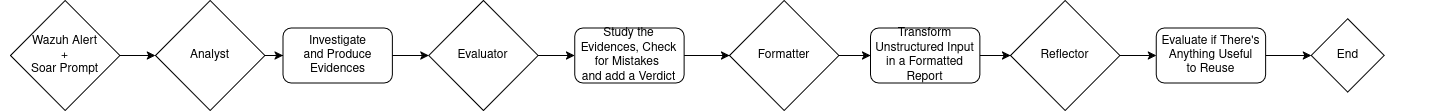
\includegraphics[keepaspectratio]{Pipeline.drawio.png}}
\caption{Agent Pipeline}
\end{figure}

The four core design goals are: 1. Deterministic orchestration with
explicit state transitions. 2. Strict interface contracts between
components. 3. Decoder-aware enrichment to avoid silent field
mismatches. 4. Progressive self-improvement through controlled memory.

\subsubsection{4.2 End-to-End State Model and LangGraph
Orchestration}\label{end-to-end-state-model-and-langgraph-orchestration}

The orchestration backbone is implemented in \texttt{agent/graph.py}
through a typed \texttt{PipelineState}. This state object is
intentionally minimal: it stores alert input, intermediate documents,
final report, skill execution log, and reflector output.

\begin{Shaded}
\begin{Highlighting}[]
\KeywordTok{class}\NormalTok{ PipelineState(TypedDict, total}\OperatorTok{=}\VariableTok{False}\NormalTok{):}
\NormalTok{    run\_id: }\BuiltInTok{str}
\NormalTok{    alert: }\BuiltInTok{dict}\NormalTok{[}\BuiltInTok{str}\NormalTok{, Any]}
\NormalTok{    soar\_prompt: }\BuiltInTok{str}
\NormalTok{    analyst\_doc: }\BuiltInTok{str}
\NormalTok{    evaluator\_doc: }\BuiltInTok{str}
\NormalTok{    report: IncidentReport}
\NormalTok{    skill\_log: }\BuiltInTok{list}\NormalTok{[SkillExecutionRecord]}
\NormalTok{    reflection: }\BuiltInTok{dict}\NormalTok{[}\BuiltInTok{str}\NormalTok{, Any]}
\end{Highlighting}
\end{Shaded}

Graph assembly is explicit and linear. The reflector node is optional,
but in the production path it is appended after formatting so it can
read the final verdict before deciding what to persist.

\begin{Shaded}
\begin{Highlighting}[]
\NormalTok{graph.add\_edge(START, }\StringTok{"analyst"}\NormalTok{)}
\NormalTok{graph.add\_edge(}\StringTok{"analyst"}\NormalTok{, }\StringTok{"evaluator"}\NormalTok{)}
\NormalTok{graph.add\_edge(}\StringTok{"evaluator"}\NormalTok{, }\StringTok{"formatter"}\NormalTok{)}
\NormalTok{graph.add\_edge(}\StringTok{"formatter"}\NormalTok{, }\StringTok{"reflector"}\NormalTok{)}
\NormalTok{graph.add\_edge(}\StringTok{"reflector"}\NormalTok{, END)}
\end{Highlighting}
\end{Shaded}

This explicit graph provides two benefits crucial for a thesis artifact:
1. Execution semantics are visible in architecture diagrams and code. 2.
Behavior changes require structural edits, not hidden prompt side
effects.

A concise sequence view of one run is shown below.

\begin{figure}
\centering
\pandocbounded{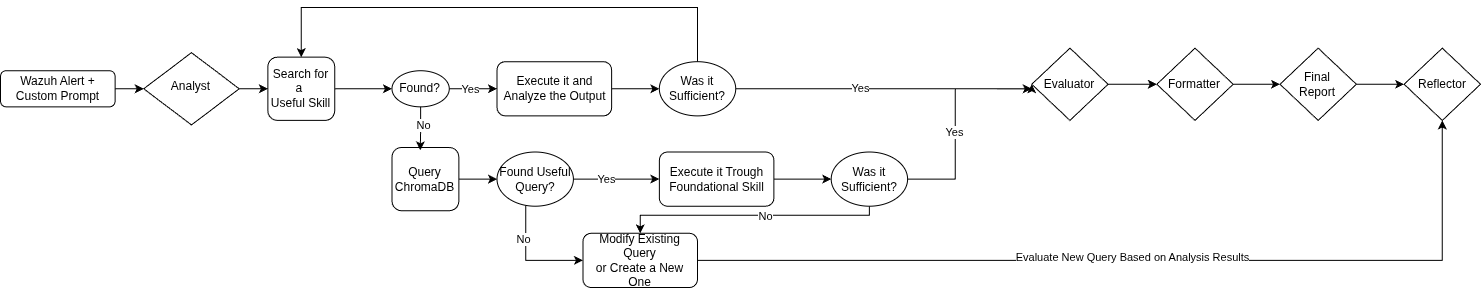
\includegraphics[keepaspectratio]{Architettura.drawio.png}}
\caption{Logic Flowchart of an Analysis}
\end{figure}

\subsubsection{4.3 Skill Contract and Execution
Lifecycle}\label{skill-contract-and-execution-lifecycle}

All skills inherit from the same abstract base in
\texttt{skills/base.py}. The contract separates private analytical logic
(\texttt{\_run}) from public runtime concerns (\texttt{execute}). This
abstract all the internal logic away from the agent, only exposing the
necessary interfaces preserving the context.

\begin{Shaded}
\begin{Highlighting}[]
\KeywordTok{class}\NormalTok{ Skill(ABC):}
\NormalTok{    name: }\BuiltInTok{str}
\NormalTok{    description: }\BuiltInTok{str}
\NormalTok{    input\_type: InputType}
\NormalTok{    is\_generic: }\BuiltInTok{bool} \OperatorTok{=} \VariableTok{False}
\NormalTok{    tool\_input\_schema: }\BuiltInTok{dict}\NormalTok{[}\BuiltInTok{str}\NormalTok{, Any] }\OperatorTok{|} \VariableTok{None} \OperatorTok{=} \VariableTok{None}

    \AttributeTok{@abstractmethod}
    \KeywordTok{def}\NormalTok{ \_run(}\VariableTok{self}\NormalTok{, value: }\BuiltInTok{str}\NormalTok{, context: }\BuiltInTok{dict}\NormalTok{[}\BuiltInTok{str}\NormalTok{, Any]) }\OperatorTok{{-}\textgreater{}}\NormalTok{ SkillResult:}
\NormalTok{        ...}

    \KeywordTok{def}\NormalTok{ execute(}\VariableTok{self}\NormalTok{, value: }\BuiltInTok{str}\NormalTok{, context: }\BuiltInTok{dict}\NormalTok{[}\BuiltInTok{str}\NormalTok{, Any] }\OperatorTok{|} \VariableTok{None} \OperatorTok{=} \VariableTok{None}\NormalTok{) }\OperatorTok{{-}\textgreater{}}\NormalTok{ SkillResult:}
        \CommentTok{\# wraps \_run with timing + top{-}level exception guard}
\end{Highlighting}
\end{Shaded}

The \texttt{SkillResult} structure is shared by all skills and
explicitly stores both machine-usable payload and analyst-readable
summary.

\begin{Shaded}
\begin{Highlighting}[]
\AttributeTok{@dataclass}
\KeywordTok{class}\NormalTok{ SkillResult:}
\NormalTok{    data: }\BuiltInTok{dict}\NormalTok{[}\BuiltInTok{str}\NormalTok{, Any]}
\NormalTok{    summary: }\BuiltInTok{str}
\NormalTok{    success: }\BuiltInTok{bool}
\NormalTok{    source: }\BuiltInTok{str} \OperatorTok{=} \StringTok{""}
\NormalTok{    duration\_ms: }\BuiltInTok{float} \OperatorTok{=} \FloatTok{0.0}
\end{Highlighting}
\end{Shaded}

Execution lifecycle of one skill call: 1. Analyst issues tool
invocation. 2. Skill receives \texttt{value} plus shared
\texttt{context}. 3. \texttt{\_run} executes domain logic and returns
\texttt{SkillResult}. 4. \texttt{execute} stamps source and duration,
catches unhandled exceptions. 5. Result is serialized back to the agent
loop as tool output.

This lifecycle creates uniform execution flow and simplifies regression
testing across heterogeneous skills.

\subsubsection{4.4 Skill Registry and Discovery
Architecture}\label{skill-registry-and-discovery-architecture}

The registry in \texttt{skills/registry.py} stores ready-to-run skill
instances, not classes. The choice of dependency-injection here is
deliberate since each skill can receive pre-wired collaborators
(builder, executor, store, LLM client) during startup, then be reused at
runtime without reconstruction.

\begin{Shaded}
\begin{Highlighting}[]
\KeywordTok{class}\NormalTok{ SkillRegistry:}
\NormalTok{    \_instance: }\StringTok{"SkillRegistry | None"} \OperatorTok{=} \VariableTok{None}

    \KeywordTok{def}\NormalTok{ register(}\VariableTok{self}\NormalTok{, skill: Skill) }\OperatorTok{{-}\textgreater{}} \VariableTok{None}\NormalTok{:}
        \VariableTok{self}\NormalTok{.\_skills[skill.name] }\OperatorTok{=}\NormalTok{ skill}

    \KeywordTok{def}\NormalTok{ get(}\VariableTok{self}\NormalTok{, name: }\BuiltInTok{str}\NormalTok{) }\OperatorTok{{-}\textgreater{}}\NormalTok{ Skill }\OperatorTok{|} \VariableTok{None}\NormalTok{:}
        \ControlFlowTok{return} \VariableTok{self}\NormalTok{.\_skills.get(name)}
\end{Highlighting}
\end{Shaded}

Analysis skills are auto-discovered by scanning
\texttt{skills/analysis/} modules and selecting concrete \texttt{Skill}
subclasses whose \texttt{input\_type} is not foundational.

\begin{Shaded}
\begin{Highlighting}[]
\KeywordTok{def}\NormalTok{ discover\_skill\_classes() }\OperatorTok{{-}\textgreater{}} \BuiltInTok{list}\NormalTok{[}\BuiltInTok{type}\NormalTok{[Skill]]:}
    \CommentTok{\# import every module in skills.analysis}
    \CommentTok{\# collect concrete Skill subclasses}
\end{Highlighting}
\end{Shaded}

Foundational generic skills (\texttt{chroma\_query},
\texttt{query\_crafter}) are wired manually in \texttt{agent/runner.py}
because they require explicit dependencies that auto-discovery cannot
infer safely.

\begin{Shaded}
\begin{Highlighting}[]
\NormalTok{registry.register(}
\NormalTok{    ChromaQuerySkill(}
\NormalTok{        client}\OperatorTok{=}\NormalTok{anthropic\_client,}
\NormalTok{        store}\OperatorTok{=}\NormalTok{chroma\_store,}
\NormalTok{        executor}\OperatorTok{=}\NormalTok{executor,}
\NormalTok{    )}
\NormalTok{)}
\NormalTok{registry.register(}
\NormalTok{    QueryCrafterSkill(}
\NormalTok{        client}\OperatorTok{=}\NormalTok{anthropic\_client,}
\NormalTok{        executor}\OperatorTok{=}\NormalTok{executor,}
\NormalTok{    )}
\NormalTok{)}
\end{Highlighting}
\end{Shaded}

\subsubsection{4.5 Decoder-Specific Analysis-Skill
Strategy}\label{decoder-specific-analysis-skill-strategy}

A central design decision is to use one skill family per
decoder/log-source semantic. This inevitably leads to more human work to
prepare a sufficient number of skill instances. The main reason for this
choice is that different decoders map the same logical fields to
different variables. For example, an IP address is
\texttt{data.win.eventdata.ipAddress} in Windows logs, but it could be
\texttt{data.srcIp} in a firewall log. A generic skill would have to
guess which field to query, and if it guessed wrong it would return zero
results without any explicit error. Another option would be to rewrite
built-in and custom decoders to map the same logical field to common
variables, but this would require substantial maintenance, would be
error-prone, and could be impossible when source logs contain highly
specific fields.

The current implementation provides a Windows decoder set: 1.
\texttt{windows\_ip\_lookup} 2. \texttt{windows\_username\_lookup} 3.
\texttt{windows\_rule\_lookup}

Each skill defines a source-specific OpenSearch template and aggregates
only relevant fields. For example, \texttt{windows\_ip\_lookup} targets
\texttt{data.win.eventdata.ipAddress} with an explicit decoder filter:

\begin{Shaded}
\begin{Highlighting}[]
\FunctionTok{\{}
  \DataTypeTok{"query"}\FunctionTok{:} \FunctionTok{\{}
    \DataTypeTok{"bool"}\FunctionTok{:} \FunctionTok{\{}
      \DataTypeTok{"filter"}\FunctionTok{:} \OtherTok{[}
        \FunctionTok{\{}\DataTypeTok{"term"}\FunctionTok{:} \FunctionTok{\{}\DataTypeTok{"data.win.eventdata.ipAddress"}\FunctionTok{:} \FunctionTok{\{}\ErrorTok{\{ip\_address}\FunctionTok{\}\}\}}\ErrorTok{\}}\OtherTok{,}
        \FunctionTok{\{}\DataTypeTok{"term"}\FunctionTok{:} \FunctionTok{\{}\DataTypeTok{"decoder.name"}\FunctionTok{:} \StringTok{"windows\_eventchannel"}\FunctionTok{\}\}}
      \OtherTok{]}
    \FunctionTok{\}}
  \FunctionTok{\}}
\FunctionTok{\}}
\end{Highlighting}
\end{Shaded}

It also aggregates only the fields relevant for IP analysis, avoiding
unnecessary token consumption:

\begin{Shaded}
\begin{Highlighting}[]
\FunctionTok{\{}
  \DataTypeTok{"aggs"}\FunctionTok{:} \FunctionTok{\{}
    \DataTypeTok{"activity\_over\_time"}\FunctionTok{:} \FunctionTok{\{}
      \DataTypeTok{"date\_histogram"}\FunctionTok{:} \FunctionTok{\{}
        \DataTypeTok{"field"}\FunctionTok{:} \StringTok{"@timestamp"}\FunctionTok{,}
        \DataTypeTok{"fixed\_interval"}\FunctionTok{:} \StringTok{"5m"}\FunctionTok{,}
        \DataTypeTok{"min\_doc\_count"}\FunctionTok{:} \DecValTok{1}
      \FunctionTok{\}}
    \FunctionTok{\},}
    \DataTypeTok{"top\_rules"}\FunctionTok{:} \FunctionTok{\{}
      \DataTypeTok{"terms"}\FunctionTok{:} \FunctionTok{\{}\DataTypeTok{"field"}\FunctionTok{:} \StringTok{"rule.id"}\FunctionTok{,} \DataTypeTok{"size"}\FunctionTok{:} \DecValTok{5}\FunctionTok{\},}
      \DataTypeTok{"aggs"}\FunctionTok{:} \FunctionTok{\{}
        \DataTypeTok{"rule\_meta"}\FunctionTok{:} \FunctionTok{\{}
          \DataTypeTok{"top\_hits"}\FunctionTok{:} \FunctionTok{\{}\DataTypeTok{"size"}\FunctionTok{:} \DecValTok{1}\FunctionTok{,} \DataTypeTok{"\_source"}\FunctionTok{:} \OtherTok{[}\StringTok{"rule.level"}\OtherTok{,} \StringTok{"rule.description"}\OtherTok{]}\FunctionTok{\}}
        \FunctionTok{\}}
      \FunctionTok{\}}
    \FunctionTok{\},}
    \DataTypeTok{"top\_users"}\FunctionTok{:} \FunctionTok{\{}
      \DataTypeTok{"terms"}\FunctionTok{:} \FunctionTok{\{}\DataTypeTok{"field"}\FunctionTok{:} \StringTok{"data.win.eventdata.targetUserName"}\FunctionTok{,} \DataTypeTok{"size"}\FunctionTok{:} \DecValTok{5}\FunctionTok{\}}
    \FunctionTok{\},}
    \DataTypeTok{"top\_dst\_ips"}\FunctionTok{:} \FunctionTok{\{}
      \DataTypeTok{"terms"}\FunctionTok{:} \FunctionTok{\{}\DataTypeTok{"field"}\FunctionTok{:} \StringTok{"data.win.eventdata.destinationAddress"}\FunctionTok{,} \DataTypeTok{"size"}\FunctionTok{:} \DecValTok{5}\FunctionTok{\}}
    \FunctionTok{\},}
    \DataTypeTok{"top\_dst\_ports"}\FunctionTok{:} \FunctionTok{\{}
      \DataTypeTok{"terms"}\FunctionTok{:} \FunctionTok{\{}\DataTypeTok{"field"}\FunctionTok{:} \StringTok{"data.win.eventdata.destinationPort"}\FunctionTok{,} \DataTypeTok{"size"}\FunctionTok{:} \DecValTok{5}\FunctionTok{\}}
    \FunctionTok{\}}
  \FunctionTok{\}}
\FunctionTok{\}}
\end{Highlighting}
\end{Shaded}

This strategy improves correctness and interpretability: 1. Query intent
is explicit per source. 2. Empty results are less likely to come from
schema mismatch. 3. Skill descriptions remain operationally meaningful
for the analyst LLM. 4. It's easier for the Analyst to identify which
skill to use for each source, improving tool-use precision.

\subsubsection{4.6 Layered Query Pipeline and Dependency
Boundaries}\label{layered-query-pipeline-and-dependency-boundaries}

Data access follows a strict three-layer path:

\begin{figure}
\centering
\pandocbounded{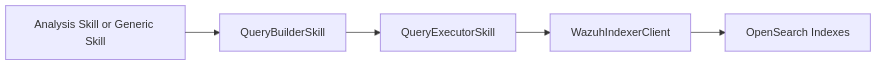
\includegraphics[keepaspectratio]{image.png}}
\caption{Data Access Pipeline}
\end{figure}

This separation is enforced in code: 1. \texttt{QueryBuilderSkill}
performs deterministic template substitution. 2.
\texttt{QueryExecutorSkill} validates DSL JSON and executes queries. 3.
\texttt{WazuhIndexerClient} encapsulates OpenSearch connectivity and
auth.

Builder substitution uses JSON-safe replacement for placeholders:

\begin{Shaded}
\begin{Highlighting}[]
\KeywordTok{def}\NormalTok{ \_substitute(template: }\BuiltInTok{str}\NormalTok{, params: }\BuiltInTok{dict}\NormalTok{[}\BuiltInTok{str}\NormalTok{, Any]) }\OperatorTok{{-}\textgreater{}} \BuiltInTok{str}\NormalTok{:}
    \KeywordTok{def}\NormalTok{ \_replacer(match: re.Match) }\OperatorTok{{-}\textgreater{}} \BuiltInTok{str}\NormalTok{:}
        \ControlFlowTok{return}\NormalTok{ json.dumps(params[match.group(}\DecValTok{1}\NormalTok{)], separators}\OperatorTok{=}\NormalTok{(}\StringTok{","}\NormalTok{, }\StringTok{":"}\NormalTok{))}
    \ControlFlowTok{return}\NormalTok{ re.sub(}\VerbatimStringTok{r"}\CharTok{\textbackslash{}\{\textbackslash{}\{}\KeywordTok{(}\DecValTok{\textbackslash{}w}\OperatorTok{+}\KeywordTok{)}\CharTok{\textbackslash{}\}\textbackslash{}\}}\VerbatimStringTok{"}\NormalTok{, \_replacer, template)}
\end{Highlighting}
\end{Shaded}

Executor validates query structure before sending traffic to the
indexer:

\begin{Shaded}
\begin{Highlighting}[]
\ControlFlowTok{try}\NormalTok{:}
\NormalTok{    dsl }\OperatorTok{=}\NormalTok{ json.loads(value)}
\ControlFlowTok{except}\NormalTok{ json.JSONDecodeError }\ImportTok{as}\NormalTok{ exc:}
    \ControlFlowTok{return}\NormalTok{ SkillResult.fail(}\SpecialStringTok{f"Invalid DSL — not valid JSON: }\SpecialCharTok{\{}\NormalTok{exc}\SpecialCharTok{\}}\SpecialStringTok{"}\NormalTok{)}
\end{Highlighting}
\end{Shaded}

Client-side entrypoint to OpenSearch is intentionally thin and explicit:

\begin{Shaded}
\begin{Highlighting}[]
\KeywordTok{def}\NormalTok{ execute\_query(}\VariableTok{self}\NormalTok{, query: }\BuiltInTok{dict}\NormalTok{[}\BuiltInTok{str}\NormalTok{, Any], index: }\BuiltInTok{str} \OperatorTok{=}\NormalTok{ DEFAULT\_INDEX, size: }\BuiltInTok{int} \OperatorTok{=} \DecValTok{100}\NormalTok{) }\OperatorTok{{-}\textgreater{}} \BuiltInTok{dict}\NormalTok{[}\BuiltInTok{str}\NormalTok{, Any]:}
    \ControlFlowTok{return} \VariableTok{self}\NormalTok{.\_client.search(body}\OperatorTok{=}\NormalTok{query, index}\OperatorTok{=}\NormalTok{index, size}\OperatorTok{=}\NormalTok{size)}
\end{Highlighting}
\end{Shaded}

A parser layer then strips sparse data and optionally removes
\texttt{full\_log} to reduce token overhead passed to LLM components.

\begin{Shaded}
\begin{Highlighting}[]
\KeywordTok{def}\NormalTok{ parse\_hits(}
\NormalTok{    response: }\BuiltInTok{dict}\NormalTok{[}\BuiltInTok{str}\NormalTok{, Any],}
\NormalTok{    keep\_full\_log: }\BuiltInTok{bool} \OperatorTok{=} \VariableTok{False}\NormalTok{,}
\NormalTok{) }\OperatorTok{{-}\textgreater{}}\NormalTok{ ParsedResponse:}
\NormalTok{    raw\_hits: }\BuiltInTok{list}\NormalTok{[}\BuiltInTok{dict}\NormalTok{[}\BuiltInTok{str}\NormalTok{, Any]] }\OperatorTok{=}\NormalTok{ response.get(}\StringTok{"hits"}\NormalTok{, \{\}).get(}\StringTok{"hits"}\NormalTok{, [])}
\NormalTok{    total: }\BuiltInTok{int} \OperatorTok{=}\NormalTok{ response.get(}\StringTok{"hits"}\NormalTok{, \{\}).get(}\StringTok{"total"}\NormalTok{, \{\}).get(}\StringTok{"value"}\NormalTok{, }\DecValTok{0}\NormalTok{)}
\NormalTok{    took\_ms: }\BuiltInTok{int} \OperatorTok{=}\NormalTok{ response.get(}\StringTok{"took"}\NormalTok{, }\DecValTok{0}\NormalTok{)}

\NormalTok{    hits: }\BuiltInTok{list}\NormalTok{[}\BuiltInTok{dict}\NormalTok{[}\BuiltInTok{str}\NormalTok{, Any]] }\OperatorTok{=}\NormalTok{ []}
    \ControlFlowTok{for}\NormalTok{ hit }\KeywordTok{in}\NormalTok{ raw\_hits:}
\NormalTok{        source: }\BuiltInTok{dict}\NormalTok{[}\BuiltInTok{str}\NormalTok{, Any] }\OperatorTok{=} \BuiltInTok{dict}\NormalTok{(hit.get(}\StringTok{"\_source"}\NormalTok{, \{\}))}
        \ControlFlowTok{if} \KeywordTok{not}\NormalTok{ keep\_full\_log:}
\NormalTok{            source.pop(}\StringTok{"full\_log"}\NormalTok{, }\VariableTok{None}\NormalTok{)}
\NormalTok{        hits.append(strip\_empty(source))}

    \ControlFlowTok{return}\NormalTok{ ParsedResponse(hits}\OperatorTok{=}\NormalTok{hits, total}\OperatorTok{=}\NormalTok{total, took\_ms}\OperatorTok{=}\NormalTok{took\_ms)}
\end{Highlighting}
\end{Shaded}

\subsubsection{4.7 Multi-Agent Pipeline: Analyst, Evaluator, Formatter,
Reflector}\label{multi-agent-pipeline-analyst-evaluator-formatter-reflector}

\paragraph{4.7.1 Analyst Agent}\label{analyst-agent}

The Analyst performs iterative evidence gathering via Anthropic tool-use
and stops when enough context is collected or a max-iteration guard is
reached.

\begin{Shaded}
\begin{Highlighting}[]
\ControlFlowTok{for}\NormalTok{ \_ }\KeywordTok{in} \BuiltInTok{range}\NormalTok{(\_MAX\_ITERATIONS):}
\NormalTok{    response }\OperatorTok{=} \VariableTok{self}\NormalTok{.\_client.messages.create(...)}
    \ControlFlowTok{if}\NormalTok{ response.stop\_reason }\OperatorTok{!=} \StringTok{"tool\_use"}\NormalTok{:}
        \ControlFlowTok{break}
\end{Highlighting}
\end{Shaded}

Tool exposure is controlled by decoder prefix plus generic-skill
override:

\begin{Shaded}
\begin{Highlighting}[]
\ControlFlowTok{if} \BuiltInTok{getattr}\NormalTok{(skill, }\StringTok{"is\_generic"}\NormalTok{, }\VariableTok{False}\NormalTok{) }\KeywordTok{is} \VariableTok{True}\NormalTok{:}
    \ControlFlowTok{return} \VariableTok{True}
\ControlFlowTok{return}\NormalTok{ skill.name.startswith(prefix)}
\end{Highlighting}
\end{Shaded}

The possibility of multiple analyst agents was explored, but excluded
for reducing complexity. Future work could explore more specialized
analyst roles, but for this thesis the single Analyst agent is
sufficient to test the core research questions about LLM-based
investigation pipelines.

\paragraph{4.7.2 Evaluator Agent}\label{evaluator-agent}

The Evaluator receives only the analyst document and performs verdict
reasoning (\texttt{true\_positive}, \texttt{false\_positive},
\texttt{inconclusive}) with a confidence score. It has no tool access by
design. This forces it to make a judgment based solely on the evidence
collected by the Analyst, without any possibility of further information
gathering. This design choice is intentional to create a clear
separation between evidence collection and verdict reasoning, which
simplifies both the architecture and the evaluation of the system's
performance on these distinct tasks.

\paragraph{4.7.3 Formatter Agent}\label{formatter-agent}

The Formatter enforces schema consistency by forcing a single
\texttt{produce\_report} tool call. This avoids relying on fragile
free-form generation for structured outputs. Note that both the analyst
and the evaluator are instructed to produce semi-structured text, but
only the formatter is required to produce a fixed-schema report. This
allows the analyst and evaluator to express their reasoning in a more
natural way, while still ensuring that the final output is consistent
and machine-readable.

\begin{Shaded}
\begin{Highlighting}[]
\NormalTok{response }\OperatorTok{=} \VariableTok{self}\NormalTok{.\_client.messages.create(}
\NormalTok{    tools}\OperatorTok{=}\NormalTok{[PRODUCE\_REPORT\_TOOL],}
\NormalTok{    tool\_choice}\OperatorTok{=}\NormalTok{\{}\StringTok{"type"}\NormalTok{: }\StringTok{"any"}\NormalTok{\},}
\NormalTok{    ...}
\NormalTok{)}
\end{Highlighting}
\end{Shaded}

\paragraph{4.7.4 Reflector Agent}\label{reflector-agent}

The Reflector is executed after formatting and uses
\texttt{skill\_log\ +\ evaluator\_doc} to apply memory policy decisions.
It does not modify the final report; it only performs persistence side
effects and in case add the query to the knowledge store.

\begin{Shaded}
\begin{Highlighting}[]
\KeywordTok{def}\NormalTok{ \_promote(}\VariableTok{self}\NormalTok{, record: }\BuiltInTok{dict}\NormalTok{[}\BuiltInTok{str}\NormalTok{, Any]) }\OperatorTok{{-}\textgreater{}} \BuiltInTok{str} \OperatorTok{|} \VariableTok{None}\NormalTok{:}
    \ControlFlowTok{try}\NormalTok{:}
\NormalTok{        description, goal }\OperatorTok{=} \VariableTok{self}\NormalTok{.\_describe(record)}
    \ControlFlowTok{except} \PreprocessorTok{Exception}\NormalTok{:}
        \CommentTok{\# Describe failure should not crash the pipeline — fall back to}
        \CommentTok{\# the analyst\textquotesingle{}s original goal as both fields.}
\NormalTok{        description }\OperatorTok{=}\NormalTok{ record.get(}\StringTok{"goal"}\NormalTok{, }\StringTok{""}\NormalTok{)}
\NormalTok{        goal }\OperatorTok{=}\NormalTok{ record.get(}\StringTok{"goal"}\NormalTok{, }\StringTok{""}\NormalTok{)}

\NormalTok{    stored }\OperatorTok{=}\NormalTok{ StoredQuery(}
\NormalTok{        description}\OperatorTok{=}\NormalTok{description,}
\NormalTok{        query}\OperatorTok{=}\NormalTok{record.get(}\StringTok{"crafted\_dsl"}\NormalTok{, }\StringTok{""}\NormalTok{),}
\NormalTok{        parameters}\OperatorTok{=}\BuiltInTok{list}\NormalTok{(record.get(}\StringTok{"parameters"}\NormalTok{, [])),}
\NormalTok{        security\_component}\OperatorTok{=}\NormalTok{record.get(}\StringTok{"security\_component"}\NormalTok{, }\StringTok{""}\NormalTok{),}
\NormalTok{        sec\_comp\_extra}\OperatorTok{=}\NormalTok{record.get(}\StringTok{"sec\_comp\_extra"}\NormalTok{, }\StringTok{""}\NormalTok{),}
\NormalTok{        input\_type}\OperatorTok{=}\NormalTok{record.get(}\StringTok{"input\_type"}\NormalTok{, }\StringTok{""}\NormalTok{),}
\NormalTok{        goal}\OperatorTok{=}\NormalTok{goal,}
\NormalTok{    )}
    \VariableTok{self}\NormalTok{.\_store.add(stored)}
    \ControlFlowTok{return}\NormalTok{ stored.}\BuiltInTok{id}
\end{Highlighting}
\end{Shaded}

\subsubsection{4.8 Knowledge Memory and Reflection
Policy}\label{knowledge-memory-and-reflection-policy}

Knowledge accumulation is implemented through ChromaDB in
\texttt{store/chroma\_client.py} and two generic skills: 1.
\texttt{ChromaQuerySkill} (retrieve and execute past queries) 2.
\texttt{QueryCrafterSkill} (generate and validate novel queries)

\paragraph{4.8.1 Chroma Schema and
Retrieval}\label{chroma-schema-and-retrieval}

Stored query records include both DSL and operational metadata:

\begin{Shaded}
\begin{Highlighting}[]
\AttributeTok{@dataclass}
\KeywordTok{class}\NormalTok{ StoredQuery:}
\NormalTok{    description: }\BuiltInTok{str}
\NormalTok{    query: }\BuiltInTok{str}
\NormalTok{    parameters: }\BuiltInTok{list}\NormalTok{[}\BuiltInTok{str}\NormalTok{]}
\NormalTok{    security\_component: }\BuiltInTok{str}
\NormalTok{    sec\_comp\_extra: }\BuiltInTok{str}
\NormalTok{    input\_type: }\BuiltInTok{str}
\NormalTok{    goal: }\BuiltInTok{str}
\NormalTok{    times\_used: }\BuiltInTok{int} \OperatorTok{=} \DecValTok{0}
\NormalTok{    times\_successful: }\BuiltInTok{int} \OperatorTok{=} \DecValTok{0}
\end{Highlighting}
\end{Shaded}

Retrieval uses strict metadata filtering before semantic similarity:

\begin{Shaded}
\begin{Highlighting}[]
\KeywordTok{def}\NormalTok{ search(}
    \VariableTok{self}\NormalTok{,}
\NormalTok{    goal: }\BuiltInTok{str}\NormalTok{,}
\NormalTok{    security\_component: }\BuiltInTok{str}\NormalTok{,}
\NormalTok{    input\_type: }\BuiltInTok{str}\NormalTok{,}
\NormalTok{    k: }\BuiltInTok{int} \OperatorTok{=} \DecValTok{3}\NormalTok{,}
\NormalTok{) }\OperatorTok{{-}\textgreater{}} \BuiltInTok{list}\NormalTok{[StoredQuery]:}
\NormalTok{    where }\OperatorTok{=}\NormalTok{ \{}
        \StringTok{"$and"}\NormalTok{: [}
\NormalTok{            \{}\StringTok{"security\_component"}\NormalTok{: \{}\StringTok{"$eq"}\NormalTok{: security\_component\}\},}
\NormalTok{            \{}\StringTok{"input\_type"}\NormalTok{: \{}\StringTok{"$eq"}\NormalTok{: input\_type\}\},}
\NormalTok{        ]}
\NormalTok{    \}}
\NormalTok{    results }\OperatorTok{=} \VariableTok{self}\NormalTok{.\_collection.query(}
\NormalTok{        query\_texts}\OperatorTok{=}\NormalTok{[goal],}
\NormalTok{        n\_results}\OperatorTok{=}\NormalTok{k,}
\NormalTok{        where}\OperatorTok{=}\NormalTok{where,}
\NormalTok{    )}
\NormalTok{    ids }\OperatorTok{=}\NormalTok{ results.get(}\StringTok{"ids"}\NormalTok{, [[]])[}\DecValTok{0}\NormalTok{]}
\NormalTok{    metadatas }\OperatorTok{=}\NormalTok{ results.get(}\StringTok{"metadatas"}\NormalTok{, [[]])[}\DecValTok{0}\NormalTok{]}
    \ControlFlowTok{return}\NormalTok{ [}
\NormalTok{        StoredQuery.from\_metadata(doc\_id}\OperatorTok{=}\NormalTok{ids[i], metadata}\OperatorTok{=}\NormalTok{metadatas[i])}
        \ControlFlowTok{for}\NormalTok{ i }\KeywordTok{in} \BuiltInTok{range}\NormalTok{(}\BuiltInTok{len}\NormalTok{(ids))}
\NormalTok{    ]}
\end{Highlighting}
\end{Shaded}

This prevents cross-context retrieval errors and keeps semantic ranking
inside a valid scope.

\paragraph{4.8.2 Query Crafting and
Validation}\label{query-crafting-and-validation}

When retrieval is insufficient, \texttt{QueryCrafterSkill} synthesizes a
new DSL via forced tool output, then validates it by live execution. A
syntax/runtime failure triggers one retry with error feedback.

\begin{Shaded}
\begin{Highlighting}[]
\KeywordTok{def}\NormalTok{ \_craft(}\VariableTok{self}\NormalTok{, user\_message: }\BuiltInTok{str}\NormalTok{) }\OperatorTok{{-}\textgreater{}} \BuiltInTok{tuple}\NormalTok{[}\BuiltInTok{str}\NormalTok{, }\BuiltInTok{list}\NormalTok{[}\BuiltInTok{str}\NormalTok{]]:}
    \CommentTok{"""Single LLM round{-}trip → \textasciigrave{}\textasciigrave{}(dsl\_string, parameter\_names)\textasciigrave{}\textasciigrave{}."""}
\NormalTok{    response }\OperatorTok{=} \VariableTok{self}\NormalTok{.\_client.messages.create(}
\NormalTok{        model}\OperatorTok{=}\VariableTok{self}\NormalTok{.\_model,}
\NormalTok{        max\_tokens}\OperatorTok{=}\DecValTok{2048}\NormalTok{,}
\NormalTok{        system}\OperatorTok{=}\NormalTok{\_SYSTEM\_PROMPT,}
\NormalTok{        tools}\OperatorTok{=}\NormalTok{[\_EMIT\_QUERY\_TOOL],}
\NormalTok{        tool\_choice}\OperatorTok{=}\NormalTok{\{}\StringTok{"type"}\NormalTok{: }\StringTok{"tool"}\NormalTok{, }\StringTok{"name"}\NormalTok{: }\StringTok{"emit\_query"}\NormalTok{\},}
\NormalTok{        messages}\OperatorTok{=}\NormalTok{[\{}\StringTok{"role"}\NormalTok{: }\StringTok{"user"}\NormalTok{, }\StringTok{"content"}\NormalTok{: user\_message\}],}
\NormalTok{    )}
    \ControlFlowTok{for}\NormalTok{ block }\KeywordTok{in}\NormalTok{ response.content:}
        \ControlFlowTok{if} \BuiltInTok{getattr}\NormalTok{(block, }\StringTok{"type"}\NormalTok{, }\VariableTok{None}\NormalTok{) }\OperatorTok{==} \StringTok{"tool\_use"} \KeywordTok{and}\NormalTok{ block.name }\OperatorTok{==} \StringTok{"emit\_query"}\NormalTok{:}
\NormalTok{            dsl }\OperatorTok{=}\NormalTok{ block.}\BuiltInTok{input}\NormalTok{.get(}\StringTok{"dsl"}\NormalTok{, }\StringTok{""}\NormalTok{)}
\NormalTok{            params }\OperatorTok{=}\NormalTok{ block.}\BuiltInTok{input}\NormalTok{.get(}\StringTok{"parameters"}\NormalTok{, [])}
            \ControlFlowTok{return}\NormalTok{ dsl, }\BuiltInTok{list}\NormalTok{(params)}
    \ControlFlowTok{raise} \PreprocessorTok{RuntimeError}\NormalTok{(}\StringTok{"Crafter model did not call emit\_query."}\NormalTok{)}
\end{Highlighting}
\end{Shaded}

A query returning zero documents is treated as valid information, not as
generation failure.

\paragraph{4.8.3 Reflector Promotion
Rules}\label{reflector-promotion-rules}

Promotion is governed centrally in \texttt{ReflectorAgent}.

\begin{Shaded}
\begin{Highlighting}[]
\ControlFlowTok{if}\NormalTok{ verdict }\OperatorTok{==} \StringTok{"true\_positive"}\NormalTok{:}
    \ControlFlowTok{return} \VariableTok{True}
\ControlFlowTok{if}\NormalTok{ verdict }\OperatorTok{==} \StringTok{"inconclusive"} \KeywordTok{and}\NormalTok{ confidence }\OperatorTok{\textgreater{}=} \FloatTok{0.6}\NormalTok{:}
    \ControlFlowTok{return} \VariableTok{True}
\ControlFlowTok{return} \VariableTok{False}
\end{Highlighting}
\end{Shaded}

For retrieved queries, counters are updated: 1. \texttt{times\_used}
always increments. 2. \texttt{times\_successful} increments only on
successful retrieval with non-zero results and \texttt{true\_positive}
verdict.

For crafted queries, promotion requires: 1. successful execution, 2.
non-zero result count, 3. favorable verdict condition (TP or
sufficiently confident inconclusive).

This separates exploration from persistence policy, improving
architectural clarity.

\subsubsection{4.9 Structured Logging and Severity
Normalization}\label{structured-logging-and-severity-normalization}

\paragraph{4.9.1 Structured Logging}\label{structured-logging}

The logging subsystem (\texttt{agent/logging\_config.py}) configures
JSON output with stdout + rotating file sink
(\texttt{logs/soc\_agent.jsonl}). Every run gets a UUID
\texttt{run\_id}, injected into each record through a logger adapter.

\begin{Shaded}
\begin{Highlighting}[]
\KeywordTok{class}\NormalTok{ \_RunIdAdapter(logging.LoggerAdapter):}
    \KeywordTok{def}\NormalTok{ process(}\VariableTok{self}\NormalTok{, msg: }\BuiltInTok{str}\NormalTok{, kwargs: }\BuiltInTok{dict}\NormalTok{[}\BuiltInTok{str}\NormalTok{, Any]) }\OperatorTok{{-}\textgreater{}} \BuiltInTok{tuple}\NormalTok{[}\BuiltInTok{str}\NormalTok{, }\BuiltInTok{dict}\NormalTok{[}\BuiltInTok{str}\NormalTok{, Any]]:}
\NormalTok{        extra }\OperatorTok{=}\NormalTok{ kwargs.setdefault(}\StringTok{"extra"}\NormalTok{, \{\})}
\NormalTok{        extra[}\StringTok{"run\_id"}\NormalTok{] }\OperatorTok{=} \VariableTok{self}\NormalTok{.extra[}\StringTok{"run\_id"}\NormalTok{]}
        \ControlFlowTok{return}\NormalTok{ msg, kwargs}
\end{Highlighting}
\end{Shaded}

At pipeline level, \texttt{run\_pipeline()} emits at least: 1.
\texttt{pipeline\_start} 2. \texttt{pipeline\_done}

While skill-level and memory-level events are available through the
skill log and reflector outputs, this run-centric logging schema enables
later metric extraction without changing core code paths.

\paragraph{4.9.2 Severity Normalization}\label{severity-normalization}

Severity normalization is implemented in \texttt{skills/base.py} via
\texttt{Severity.from\_wazuh\_level}, mapping raw Wazuh rule levels to
stable report categories.

\begin{Shaded}
\begin{Highlighting}[]
\ControlFlowTok{if}\NormalTok{ level }\OperatorTok{\textless{}=} \DecValTok{6}\NormalTok{:}
    \ControlFlowTok{return}\NormalTok{ cls.LOW}
\ControlFlowTok{if}\NormalTok{ level }\OperatorTok{\textless{}=} \DecValTok{11}\NormalTok{:}
    \ControlFlowTok{return}\NormalTok{ cls.MEDIUM}
\ControlFlowTok{if}\NormalTok{ level }\OperatorTok{\textless{}=} \DecValTok{14}\NormalTok{:}
    \ControlFlowTok{return}\NormalTok{ cls.HIGH}
\ControlFlowTok{return}\NormalTok{ cls.CRITICAL}
\end{Highlighting}
\end{Shaded}

\subsubsection{4.10 Design Rationale and
Tradeoffs}\label{design-rationale-and-tradeoffs}

The architecture chooses explicitness over maximal abstraction. It
produces strong traceability and testability, but also introduces more
components and interfaces than a monolithic prompt chain. The tradeoff
is intentional and aligned with thesis objectives.

Main advantages: 1. Clear separation of concerns and failure domains. 2.
Decoder-aware enrichment that minimizes silent false negatives. 3.
Structured, stable report outputs suitable for downstream evaluation. 4.
Controlled self-improvement without retraining.

Main costs: 1. Higher orchestration complexity. 2. More dependency
wiring during startup. 3. Greater human effort in expanding the skills.

Given the thesis constraints of explicability and traceability, this
tradeoff is acceptable. Future work could explore ways to reduce
complexity, such as automating skill generation for new decoders.

\subsubsection{4.11 Chapter Summary}\label{chapter-summary}

This chapter detailed the full architecture from state orchestration to
skill contracts, layered data access, and memory reflection policy. The
resulting system is not a generic ``LLM wrapper,'' but a modular SOC
investigation engine with explicit control flow, typed interfaces, and
persistent analytical memory. These architectural properties provide the
foundation for the implementation analysis in Chapter 5 and for the
metrics-oriented evaluation in Chapter 6.

\end{document}
